\documentclass{beamer}
\usecolortheme{whale}
\usepackage[utf8]{inputenc}
\usepackage{dirtytalk}
\usepackage{graphicx}
\graphicspath{ {./images/} }
%Information to be included in the title page:
\title{Logic and Hybrid Systems}
\author{Manasvi Saxena}
\institute{Formal Systems Lab, UIUC}
\date{}

\setbeameroption{hide notes} % Only slides
%\setbeameroption{show only notes} % Only notes
%\setbeameroption{show notes on second screen=right} % Both
\setbeamertemplate{note page}{\pagecolor{yellow!5}\insertnote}\usepackage{palatino}
\setbeamerfont{caption}{size=\scriptsize}
\begin{document}

\frame{\titlepage}

\begin{frame}
\frametitle{Hybrid Systems}

\begin{itemize}
  \item Dynamical Systems exhibiting both discrete (jump) and continuous (flow) behaviors.
  \item Serve as models of physical systems, from thermostats to trains.
  \item Continuous dynamics specified using Differential Equations.
\end{itemize}

\end{frame}

\begin{frame}
  \frametitle{Logic and Hybrid Sytems}
  \begin{itemize}
    \item Main focus - Differential Dynamic Logic for Hybrid Systems (Andre
      Platzer).
      \pause
    \item Practical deductive verification of hybrid systems.
      \pause
    \item Introduces Hybrid Program - program notation for hybrid systems.
      \pause
    \item Dynamic Logic for Hybrid Programs, a generalization of Dynamic Logic.
      \pause
    \item Suited for automation.
  \end{itemize}

\end{frame}

\begin{frame}
\frametitle{Hybrid Automata}
\begin{itemize}
  \item Commonly used to model Hybrid Systems, via Graphs.
  \item Nodes specify continuous dynamics. Edges describe discrete transitions.
  \item Intuitive, but not suitable for deductive verification.
\end{itemize}
\begin{figure}\label{fig:train-HA}
  \centering
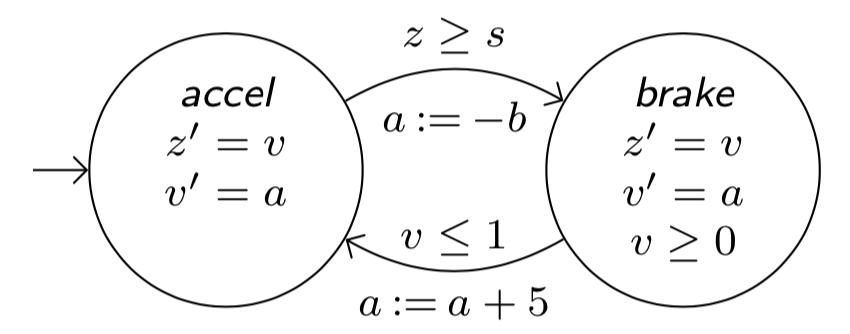
\includegraphics[scale=0.5]{train-HA}
  \caption{Hybrid Automata (simplified) of a Train Control System}
\end{figure}



\end{frame}

\end{document}

